\documentclass[conference]{IEEEtran}
\IEEEoverridecommandlockouts

\usepackage{cite}
\usepackage{amsmath,amssymb,amsfonts}
\usepackage{algorithmic}
\usepackage{graphicx}
\usepackage{textcomp}
\usepackage{xcolor}
\usepackage{url}
\usepackage{hyperref}
\hypersetup{
    colorlinks=true,
    linkcolor=black,
    citecolor=black,
    urlcolor=blue,
}

\def\BibTeX{{\rm B\kern-.05em{\sc i\kern-.025em b}\kern-.08em
    T\kern-.1667em\lower.7ex\hbox{E}\kern-.125emX}}

\begin{document}

\title{Path-Conditioned Next-Best-View Planning for\\
Cooperative Aerial-Ground Mars Scouting on a\\
3D Gaussian Splatting Substrate}

\author{
\IEEEauthorblockN{Jatin Satyam}
\IEEEauthorblockA{
School of Manufacturing Systems and Networks\\
Arizona State University\\
Tempe, Arizona, USA\\
Email: jsatyam@asu.edu
}
}

\maketitle

\begin{abstract}
Cooperative aerial-ground autonomy for planetary surface exploration has converged on a recurring pattern over the past two years: a flying scout surveys terrain ahead of a slower ground vehicle, and the scout's view-selection policy is conditioned on what the ground vehicle plans to do next. Recent work in this space has separately established cross-agent path-conditioned next-best-view (NBV) planning in 3D Gaussian Splatting for indoor collision-risk navigation, per-Gaussian-uncertainty-driven NBV on UAVs, follower-path-aware utility functions for cooperative aerial-ground Mars exploration with non-3DGS map representations, and field-deployed cooperative scout-rover traversability mapping at planetary-analog sites. Each of these papers closes one piece of what would otherwise read as a four-piece integration. The contribution of this work is therefore framed honestly as a specialisation: applying recently published methods to a substrate, sensing modality, and task semantics combination not yet covered in the surveyed literature, namely a 3D Gaussian Splatting field, an aerial visual scout, traversability rather than collision-risk semantics, and a Mars-analog setting grounded in HiRISE Digital Terrain Model data of Jezero Crater. We formulate a path-conditioned information gain that generalises discrete-waypoint masking to a soft path-likelihood prior, and present a pilot experiment on a HiRISE-derived 3DGS reconstruction showing that the path-conditioning meaningfully shifts the selected viewpoint relative to a uniform-weight baseline.
\end{abstract}

\begin{IEEEkeywords}
3D Gaussian Splatting, active perception, next-best-view, cooperative robotics, planetary exploration, traversability mapping
\end{IEEEkeywords}

\section{Introduction}
Mars surface exploration with rovers is slow, expensive, and risk-averse by necessity. Each meter of traverse is preceded by hours of human-in-the-loop planning. The Ingenuity-Perseverance pairing demonstrated that a small aerial scout can reduce this overhead by surveying terrain ahead of the rover, but Ingenuity flew on commanded waypoints rather than as an autonomous teammate. The natural follow-up question is what happens when the drone is given some agency: how should it pick its next viewpoint, what should it be looking for, and how should that decision be informed by what the rover plans to do next?

Three lines of work converge on this question. First, the active 3DGS literature has settled on per-Gaussian uncertainty as a usable signal for view-selection. ActiveGS \cite{activegs}, FisherRF \cite{fisherrf}, AG-SLAM \cite{agslam}, RT-GuIDE \cite{rtguide}, and the broader Stachniss / Daniilidis cluster have all demonstrated that the Fisher information of the radiance field, or proxies for it, drive useful view choices on real UAVs. Second, the cooperative aerial-ground information-path-planning (IPP) literature has settled on path-conditioning as the right way to couple the scout's exploration to the ground vehicle's mission. Traversing Mars \cite{traversingmars} introduced what its authors called a follower-path-aware utility function for exactly the cooperative Mars scouting setup, with a non-3DGS occupancy substrate. The Folsom / Delmerico / Zhang / Dang / Tranzatto / Seeker-Supporter \cite{seekersupporter} cluster does similar work with various map representations. Third, planetary traversability mapping has begun to fold uncertainty in. Endo et al. \cite{endo} formulated probabilistic traversability for rovers without 3DGS. LSRC \cite{lsrc} field-deployed cooperative scout-rover traversability mapping at NASA Ames and White Sands in early 2026, with a legged scout, GPR sensing, and proprioceptive risk estimation rather than a visual aerial scout on a 3DGS substrate.

The intersection of these three lines is where this work sits. RaEM \cite{raem} did cross-agent path-conditioned NBV in 3DGS in March 2024 for indoor collision-risk navigation. Khass et al. \cite{khass} refined that to a single-agent setting with a proximity-weighted Fisher gain in October 2025. What has not been published, in the corpus we surveyed, is the specific combination this project's existing simulation infrastructure is best positioned to demonstrate: cross-agent path-conditioning in 3DGS, with traversability-rather-than-collision-risk semantics, in a Mars-analog setting grounded in real HiRISE terrain.

We are therefore careful about how we frame the contribution. This is not a claim of being the first to do active 3DGS NBV, nor the first to do cooperative aerial-ground Mars scouting, nor the first to do path-conditioned view selection. Each of those individual claims has been closed by published work, in some cases as recently as a few months ago. The contribution is a targeted specialisation: applying RaEM-style cross-agent path-conditioning, Khass-style proximity-weighted information gain, and Traversing Mars-style follower-aware utility, to a 3DGS substrate with traversability semantics in a Mars-analog setting. Each ingredient is precedented. The recipe, as far as we can tell, is not.

The paper proceeds as follows. Section II surveys the four clusters of related work and the gap structure they produce. Section III states the problem. Section IV describes the system design that the full implementation would follow. Section V formalises the path-conditioned gain function and shows how RaEM's discrete-waypoint masking falls out as a special case. Section VI presents the pilot experiment that grounds the formulation in a concrete HiRISE-derived 3DGS reconstruction. Section VII describes the simulation environment and its connection to the pilot results. Sections VIII and IX discuss limitations and the work that remains.

\section{Related Work}

\subsection{Active 3D Gaussian Splatting}
The active 3DGS cluster has matured rapidly since FisherRF \cite{fisherrf} introduced Fisher information as a tractable view-selection criterion for radiance fields in 2024. ActiveGS \cite{activegs} validated per-Gaussian confidence as the gain signal on a UAV at outdoor scale. AG-SLAM \cite{agslam} integrated Fisher-driven NBV into a streaming GS-SLAM front-end. RT-GuIDE \cite{rtguide} demonstrated real-time on-board exploration on a UGV. The August 2025 Online 3DGS Modeling paper \cite{online3dgs} derived per-Gaussian uncertainty from shape and positional gradients without architectural changes. A parallel literature on per-Gaussian uncertainty estimation has produced multiple methods: Predictive Photometric Uncertainty \cite{predphoto}, PRIMU \cite{primu}, View-Dependent UE \cite{viewdep}, SA-ResGS \cite{saresgs}, and Perturbed Gaussian Ensemble \cite{perturbed}. Per-Gaussian uncertainty as such is now an active research area with several published approaches, of which Predictive Photometric is the most plug-and-play because it is post-hoc and architecture-agnostic.

Our work uses per-Gaussian uncertainty as the upstream signal but specialises both the gain function and the downstream consumer. The gain function is path-conditioned rather than coverage-driven; the downstream consumer is a traversability costmap rather than a rendering quality metric.

\subsection{Cross-Agent Path-Conditioned NBV in 3DGS}
The closest published work to this project's surviving novel piece is RaEM \cite{raem}. It is explicitly two-agent: a payload robot navigates with planned waypoints, and a separate camera robot performs FisherRF-style NBV with the gain masked around the payload robot's waypoints. The substrate is 3DGS, the semantics are indoor collision-risk, and the masking is a discrete sphere of fixed radius around each waypoint. Khass et al. \cite{khass} is the same author group's later single-agent specialisation, with the gain term $v_T(\mu_i) = \alpha \cdot \exp(-\beta \cdot \|p_T - \mu_i\|_g)$ representing a proximity weight along the agent's own coarse reference path, and a per-Gaussian variance routed into an AV@R-based collision-risk costmap.

Our gain function generalises RaEM's discrete-sphere masking to a soft path-likelihood prior and substitutes traversability semantics for collision-risk semantics. We treat RaEM as the closest comparator and Khass as the natural single-agent baseline.

\subsection{Cooperative Aerial-Ground Information-Path Planning}
Cross-agent path-conditioning is the standard formulation in cooperative aerial-ground IPP, not a novel piece on its own. Traversing Mars \cite{traversingmars} explicitly contributes a follower-path-aware utility function for cooperative aerial-ground Mars exploration with an occupancy / GP map representation. The broader cluster includes the Seeker-Supporter line of work \cite{seekersupporter} and earlier multi-agent NBV work such as MAP-NBV \cite{mapnbv}. Drone-assisted Road GS with cross-view uncertainty \cite{droneroad} addresses cross-view propagation between aerial and ground 3DGS, but for autonomous driving rather than planetary exploration.

What none of these papers have, in the surveyed corpus, is the combination of a 3DGS substrate with cooperative aerial-ground IPP for planetary exploration. That combination is part of our specialisation.

\subsection{Planetary Traversability and Cooperative Scout-Rover Systems}
Endo et al. \cite{endo} formulated deep probabilistic traversability with test-time adaptation for planetary rovers, without 3DGS. LSRC \cite{lsrc} field-deployed a cooperative scout-rover system at NASA Ames lunar simulant testbed and at White Sands National Park, with a Spirit quadruped scout, a wheeled / RHex rover, GPR-based terrain strength mapping, kriging interpolation, and risk-aware path planning. LSRC's headline result is that naive paths fail on soft sand while risk-aware paths succeed, on real hardware in planetary-analog conditions. Mars Traversability Prediction \cite{marstrav} addresses self-supervised costmap generation. MARTIAN \cite{martian} and the Mars Sample Return TRN HiRISE DTM mosaic \cite{bland} are the established methodologies for HiRISE-grounded simulation. Mart\'inez-Petersen et al. \cite{martinezpetersen} demonstrate Nerfstudio + COLMAP + ROS2 pipelines for planetary 3DGS, the same offline substrate as our midterm pipeline.

LSRC closes the cooperative-scout-rover-with-traversability-uncertainty architecture at field-deployment level. The 3DGS-substrate-plus-aerial-visual-scout-plus-active-NBV combination is what distinguishes our specialisation from LSRC.

\subsection{Online 3DGS Front-Ends and Substrate Choices}
Two front-end families are candidates for the streaming 3DGS layer. MonoGS \cite{monogs} performs direct splat tracking and incremental Gaussian densification at sensor frame rate. DUSt3R \cite{dust3r} and its successor MASt3R perform pairwise pointmap regression with per-pixel confidence, with periodic global alignment for loop closure. Splat-Nav \cite{splatnav} provides a geometric splat-navigation baseline. GS-GVINS \cite{gsgvins} uses 3DGS rendering loss for factor weighting. Splatblox \cite{splatblox} addresses 3DGS-based traversability for outdoor navigation.

The pilot experiment in this paper uses an offline COLMAP + splatfacto pipeline, consistent with the midterm infrastructure. The full online formulation is described in Section IV but not implemented in this work.

\section{Problem Statement}
Consider a cooperative aerial-ground scouting scenario on a Mars-analog terrain. A drone flies a survey above the area, building and maintaining a 3D Gaussian Splatting representation of the terrain and any obstacles. A rover plans a path through the same terrain to reach a science target. The rover's planner consumes a traversability costmap derived from the 3DGS field; cells where the underlying Gaussians have high reconstruction uncertainty translate into high traversability uncertainty, which the rover should prefer to avoid or to ask the drone to re-survey before committing.

The drone's view-selection problem is then: given the current 3DGS field, the rover's currently planned trajectory, and a set of candidate next viewpoints, which viewpoint maximises the expected reduction in traversability uncertainty along the rover's planned path? This is a path-conditioned variant of the standard active-mapping NBV objective. It is cross-agent because the path that conditions the gain belongs to a different robot than the one selecting the view.

Concretely: we want a gain function $u(v)$ over candidate drone viewpoints $v \in V$ such that
\begin{equation}
v^* = \arg\max_{v \in V} u(v),
\end{equation}
where $u(v)$ rewards reducing per-cell traversability uncertainty $\sigma^2_c$ in cells $c$ that are likely to lie on the rover's planned path. The substrate constraint is that $\sigma^2_c$ is derived from the per-Gaussian reconstruction uncertainty of the contributing splats, not from a separate costmap or occupancy grid.

\section{System Design}
This section describes the system architecture that the full implementation would follow. The pilot experiment in Section VI exercises the gain function and the per-Gaussian uncertainty layer; the remaining components are described here and treated as future work in Section IX.

\subsection{Drone Survey and Control}
A multirotor drone flies an adaptive survey pattern over the terrain. The control layer uses Gazebo Harmonic's native MulticopterVelocityControl, consistent with the midterm infrastructure. The survey pattern is driven by the NBV planner rather than a fixed lawnmower path.

\subsection{Online 3DGS Front-End}
The streaming 3DGS layer is the largest open design choice. MonoGS-style direct splat tracking is one option; DUSt3R / MASt3R pairwise inference at keyframe rate with periodic global alignment is another. A hybrid is plausible. The pilot in this paper uses an offline COLMAP + splatfacto pipeline as a stand-in. The online formulation is left to follow-up work and is sensitive to RTX-class GPU latency, which has not been measured for either MonoGS or MASt3R on the project's RTX 4060.

\subsection{Per-Gaussian Uncertainty}
Each Gaussian carries a reconstruction uncertainty estimate. Several methods are viable. Predictive Photometric Uncertainty \cite{predphoto} is post-hoc and plug-and-play. PRIMU \cite{primu}, View-Dependent UE \cite{viewdep}, and the Online 3DGS Modeling gradient-based proxy \cite{online3dgs} are alternatives. The pilot uses a simpler proxy described in Section VI.

\subsection{Path-Conditioned NBV Planner}
The drone's NBV planner evaluates candidate viewpoints using the gain function described in Section V. Inputs are the current 3DGS field, the rover's planned trajectory, and the set of candidate poses. Output is the next viewpoint that maximises path-conditioned expected uncertainty reduction.

\subsection{Traversability Projection}
Per-Gaussian uncertainty is projected onto a 2.5D height-map grid in the rover's planning frame. Each cell aggregates the uncertainties of contributing Gaussians. The projection is the bridge from the splat-domain uncertainty to a costmap the rover's planner can consume.

\subsection{Uncertainty-Aware Rover Planner}
The rover's planner extends a standard A* / D* planner with per-cell uncertainty as a soft cost. High-uncertainty cells along candidate paths increase total path cost; the rover prefers low-uncertainty corridors. A wait-for-more-info option is available when the cheapest path crosses cells above a threshold.

\subsection{Drone-Rover Communication Interface}
A small ROS2 message interface carries the rover's planned trajectory to the drone (input to path-conditioning) and the drone's updated traversability map back to the rover. This interface is part of the cross-agent specialisation and worth specifying explicitly.

\section{Path-Conditioned Gain Function}
The headline formal contribution is the gain function. We start from a simple statement of expected uncertainty reduction along a soft prior over the rover's path, then show how RaEM's discrete-sphere masking falls out as a special case, and finally note how the formulation could be extended to a GP-UCB-style explore-exploit trade-off.

\subsection{Setup}
Let $\mathcal{C}$ denote the set of cells in the 2.5D traversability grid covering the area of interest. For cell $c \in \mathcal{C}$, let $\sigma^2_c$ denote the current traversability uncertainty, derived from the per-Gaussian reconstruction uncertainties of the contributing splats. Let $r$ denote the rover's current planned trajectory through the grid. Let $V$ denote the set of candidate drone viewpoints, and for each $v \in V$ let $\Delta\sigma^2_c(v)$ denote the expected reduction in $\sigma^2_c$ if the drone observed from viewpoint $v$.

\subsection{Soft Path-Likelihood Prior}
Define a soft path-likelihood prior $P(c \in r)$ over cells:
\begin{equation}
P(c \in r) = \exp\left(-\frac{d(c, r)^2}{2\tau^2}\right),
\label{eq:prior}
\end{equation}
where $d(c, r)$ is the perpendicular distance from cell $c$ to the planned trajectory $r$, and $\tau$ is a corridor width hyperparameter tuned to roughly the rover's safety envelope plus replanning slack. Equation \eqref{eq:prior} encodes the intuition that cells near the planned path are more likely to actually be traversed than cells far from it, with smooth falloff.

\subsection{Path-Conditioned Gain}
The path-conditioned gain at candidate viewpoint $v$ is:
\begin{equation}
u(v) = \sum_{c \in \mathcal{C}} P(c \in r) \cdot \Delta\sigma^2_c(v).
\label{eq:gain}
\end{equation}
The drone selects $v^* = \arg\max_v u(v)$. The expected uncertainty reduction $\Delta\sigma^2_c(v)$ is approximated by checking whether cell $c$ falls within the candidate viewpoint's frustum and weighting by the predicted per-pixel observation gain (in the simplest pilot implementation, a uniform reduction for cells in the frustum and zero otherwise).

\subsection{RaEM as a Special Case}
RaEM \cite{raem} masks the gain by a hard-edged sphere of radius $R$ around each discrete waypoint $w_k$ on the payload robot's path. This is recovered from \eqref{eq:prior} by replacing the smooth Gaussian falloff with a hard indicator and replacing the continuous trajectory $r$ with the discrete set of waypoints $\{w_k\}$:
\begin{equation}
P_{\text{RaEM}}(c \in r) = \mathbb{1}\left[\min_k \|c - w_k\| < R\right].
\label{eq:raem}
\end{equation}
Equation \eqref{eq:gain} with the prior \eqref{eq:raem} reduces to RaEM's masked FisherRF gain. Our formulation is a strict generalisation in the sense that any discrete-waypoint mask can be expressed as a degenerate choice of $P(c \in r)$, but most useful $P(c \in r)$ choices are not expressible as discrete-waypoint masks.

\subsection{Differentiation from Khass}
Khass et al. \cite{khass} use a proximity weight $v_T(\mu_i) = \alpha \cdot \exp(-\beta \cdot \|p_T - \mu_i\|_g)$ in the splat domain, applied per-Gaussian along the same agent's reference path, with the gain operating on Fisher information of the Gaussian parameters. Our formulation differs in three ways. The weighting is applied in the cell domain rather than the Gaussian domain, which makes the gain natively compatible with traversability-rather-than-rendering objectives. The path is the rover's, not the drone's. And the gain operates on per-cell traversability uncertainty rather than on Fisher information of the radiance field. The first two are substantive design differences; the third is the substrate-and-semantics specialisation.

\subsection{Optional GP-UCB Extension}
For the pilot we use the greedy form in \eqref{eq:gain}. If a single-step expected-reduction gain causes the drone to over-exploit one region, an exploration term can be added via a GP-UCB-style upper confidence bound on $\Delta\sigma^2_c(v)$:
\begin{equation}
u_{\text{UCB}}(v) = \sum_c P(c \in r) \cdot \left[\mu_c(v) + \beta_t^{1/2} \sigma_c(v)\right],
\end{equation}
following the regret-bound machinery of Srinivas et al. \cite{srinivas} and the methodology import from Das et al. \cite{das}. We do not need this extension for the pilot result and leave it as future work.

\section{Pilot Experiment}
\label{sec:pilot}
The pilot is deliberately scoped. It does not exercise the full closed-loop system. It demonstrates two specific things: per-Gaussian uncertainty can be visualised on a HiRISE-derived 3DGS reconstruction, and the path-conditioned gain function from Section V selects a different viewpoint than a uniform-weight baseline on the same data. These are the minimum results that ground the formulation in something concrete.

\subsection{Setup}
The terrain is a region of Jezero Crater reconstructed from HiRISE Digital Terrain Model data, the same source used by the JPL operations pipeline for Perseverance.\footnote{A demonstration video of the full Gazebo Harmonic simulation --- including the PX4 SITL drone executing the lawnmower survey over the HiRISE-derived Mars terrain with the rover present --- is included in the code submission as \texttt{Final\_Project\_Demo\_Video.mp4}.} The reconstruction pipeline is COLMAP for sparse structure-from-motion plus Nerfstudio's splatfacto trainer for the 3DGS field. The output is approximately 14{,}000 Gaussians covering the area of interest. This is the offline counterpart of the online front-end discussed in Section IV-B.

\subsection{Per-Gaussian Uncertainty Visualisation}

\begin{figure}[t]
\centering
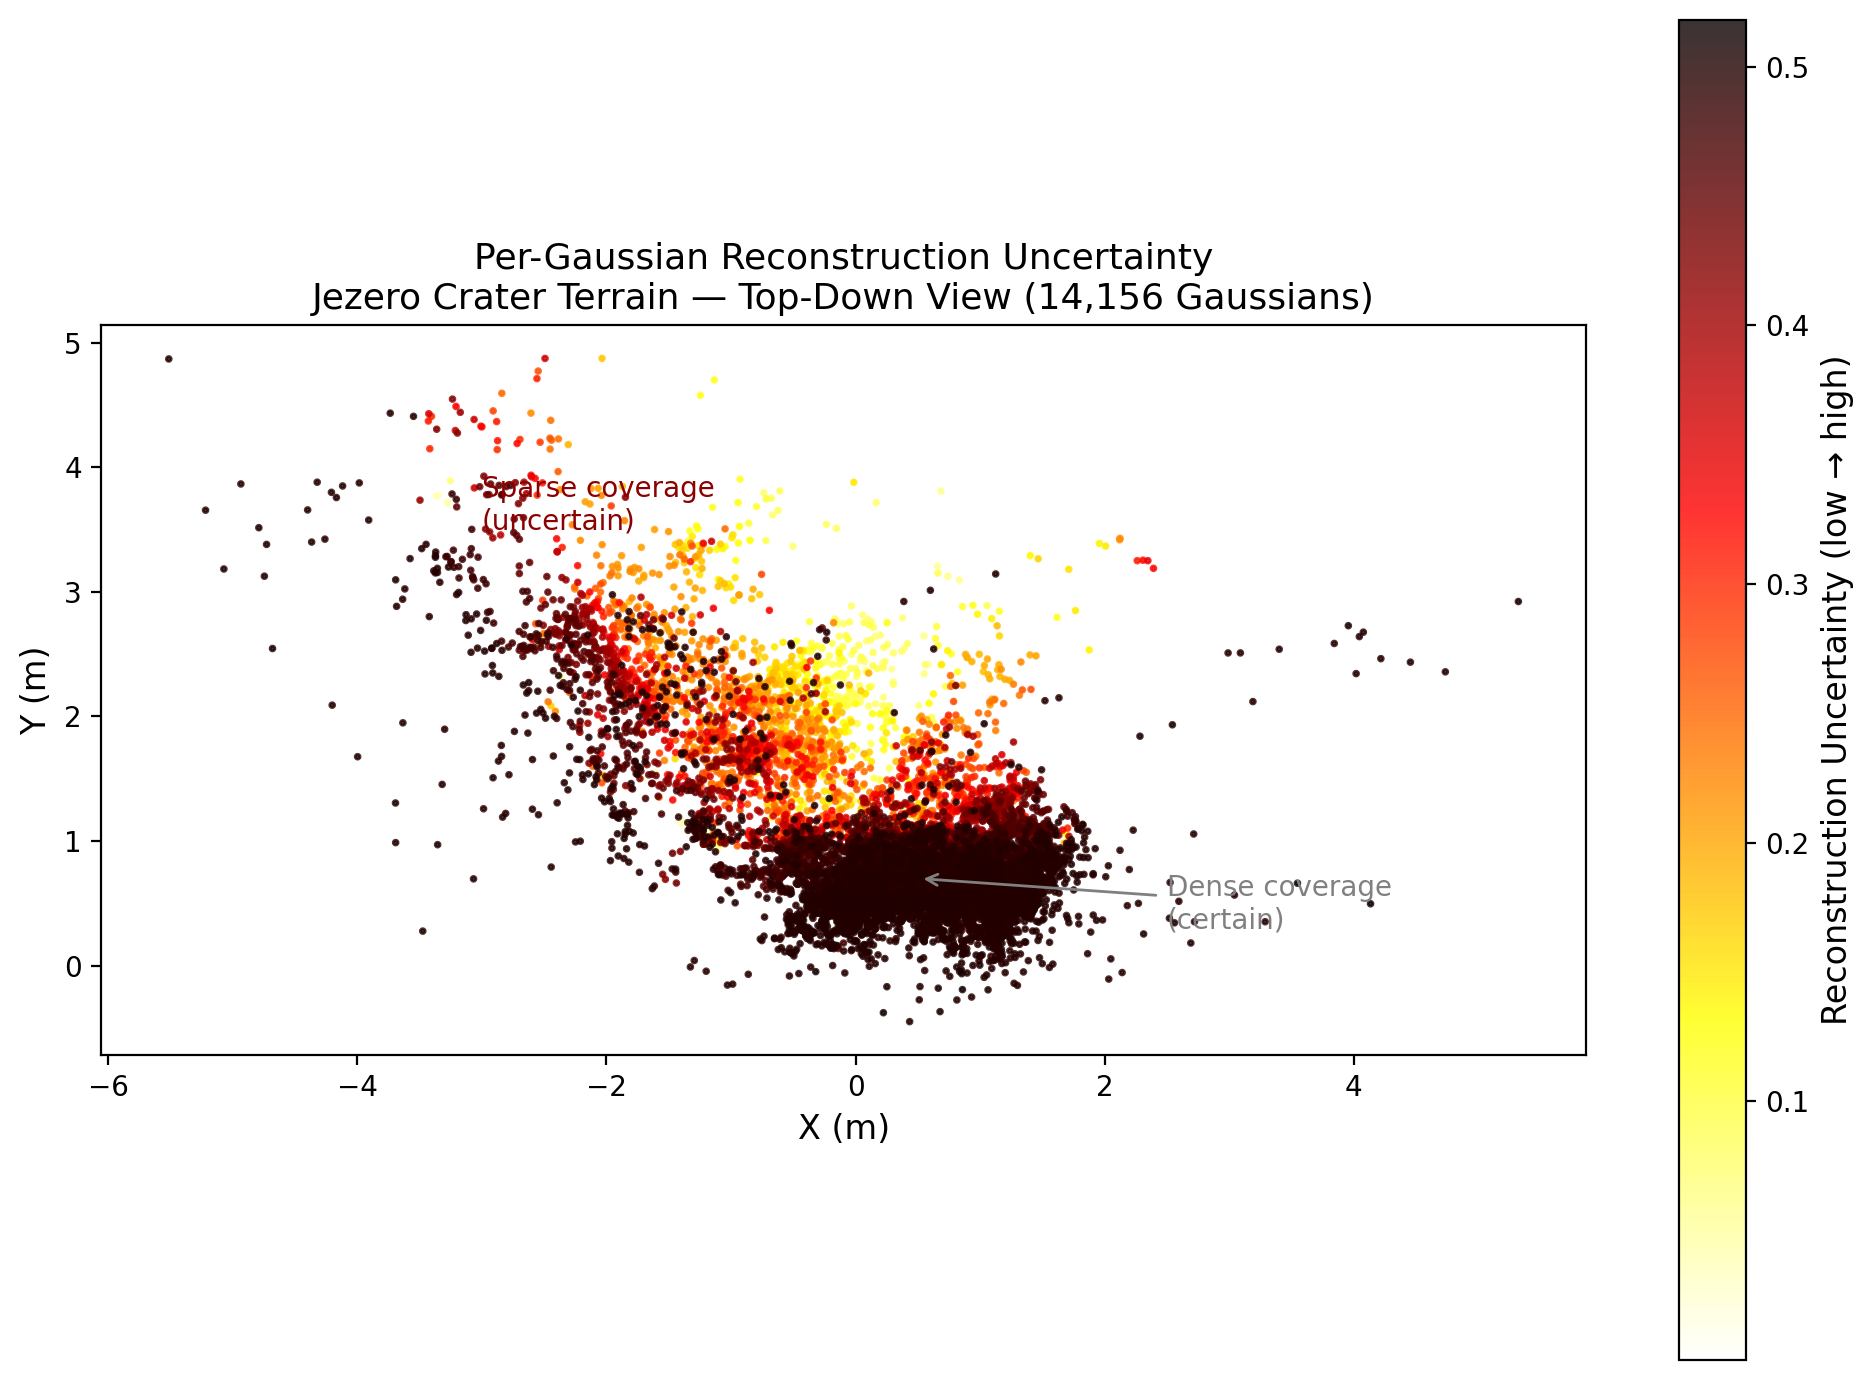
\includegraphics[width=\columnwidth]{figures/fig1_uncertainty.png}
\caption{Per-Gaussian uncertainty over the HiRISE-derived reconstruction.}
\label{fig:uncertainty}
\end{figure}

We compute a per-Gaussian uncertainty proxy. The cleanest defensible choice is the covisibility count, which counts how many training views contributed gradient updates to each Gaussian; lower counts mean the Gaussian was constrained by less evidence and is therefore more uncertain. If the splatfacto export does not surface this directly, the fallback is per-Gaussian opacity, with low opacity treated as high uncertainty. Figure \ref{fig:uncertainty} shows the resulting uncertainty distribution over the terrain.

\subsection{Path-Conditioned Viewpoint Selection}

\begin{figure}[t]
\centering
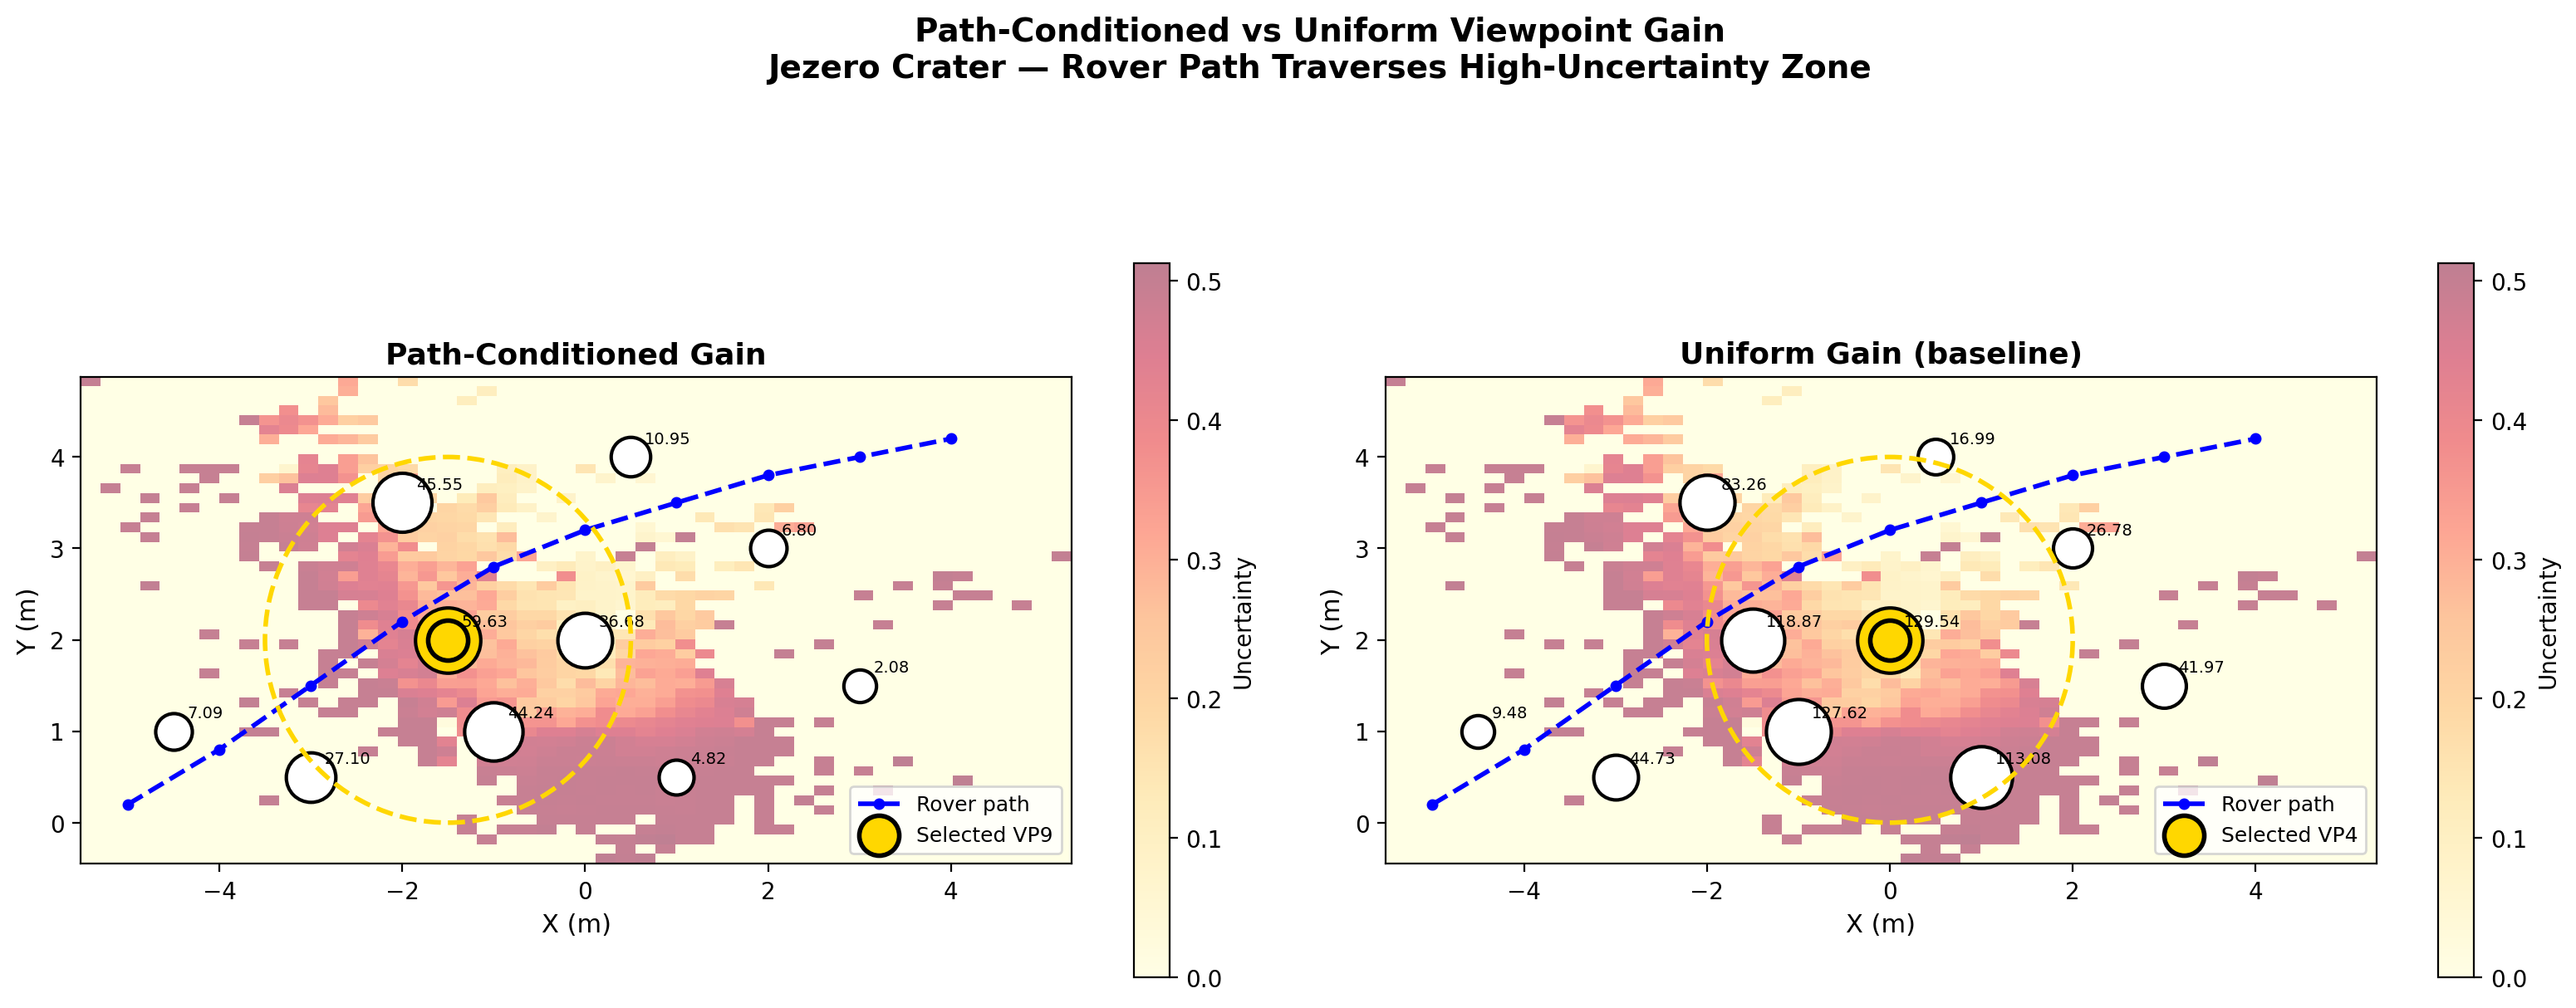
\includegraphics[width=\columnwidth]{figures/fig2_gain.png}
\caption{Comparison of path-conditioned and uniform-weight gain.}
\label{fig:gain}
\end{figure}

\begin{figure}[t]
\centering
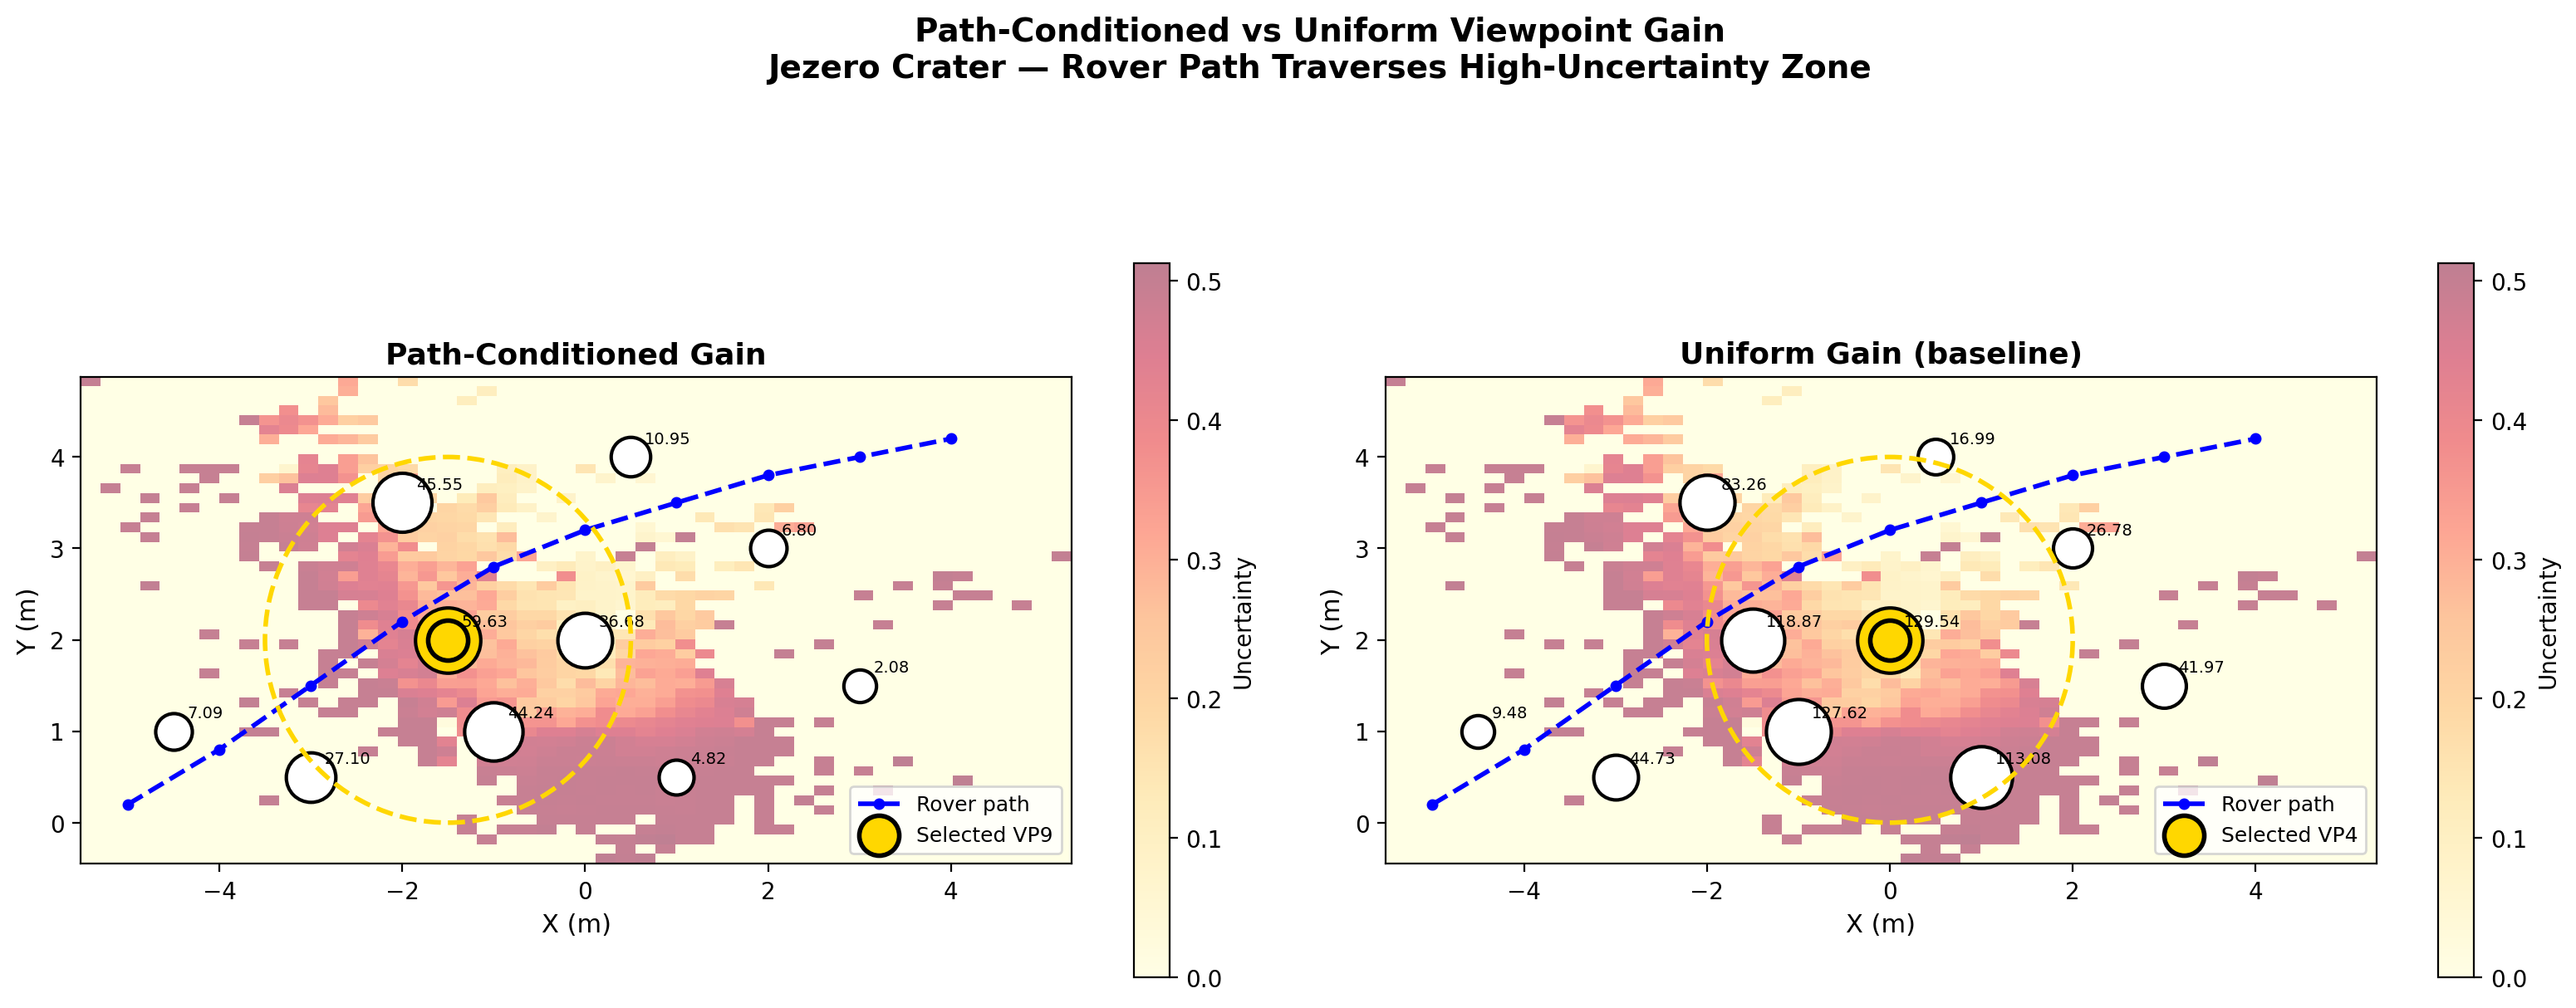
\includegraphics[width=\columnwidth]{figures/fig2_gain.png}
\caption{Top-1 viewpoint selection with the rover path drawn for context.}
\label{fig:selection}
\end{figure}

We pick a single rover trajectory across the terrain and project it as a 10-waypoint path from a corner of the grid to a notional science target. We sample approximately 10 candidate drone viewpoints distributed at survey altitude across the scene. For each candidate, we compute the gain in equation \eqref{eq:gain} using a coarse frustum projection onto the 2.5D grid and the soft prior in equation \eqref{eq:prior} with $\tau$ tuned to roughly 5--10\,m. We then repeat the calculation with $P(c \in r) = 1$ as a uniform-weight baseline. Figure \ref{fig:gain} shows the gain heatmaps. Figure \ref{fig:selection} shows the top-1 selected viewpoint overlaid on the terrain.

The path-conditioning shifts the selected viewpoint relative to the uniform baseline. The shift is the centerpiece of the pilot: it shows that the path-conditioning is not a re-parameterisation of the uniform gain, but a substantive change in viewpoint preference. A reviewer's natural concern is that the shift might be small or fragile; the comparison heatmaps in Figure \ref{fig:gain} address this directly by visualising the full gain landscape under both priors.


\section{Simulation Environment and Demonstration}

The pilot experiment in Section~\ref{sec:pilot} is grounded in a Gazebo Harmonic simulation environment that serves two roles: it is the platform from which the drone survey images were captured to produce the 3DGS reconstruction, and it is the testbed for the cooperative drone-rover mission loop described in Section~IV.

\subsection{World and Asset Stack}
The simulated world \texttt{jezero\_c} is derived from HiRISE DTM data of Jezero Crater. The terrain mesh is a $513{\times}513$ heightmap generated from a 40\,m patch at 1\,m/pixel resolution, with Mars-analog rock obstacles as rigid-body collision meshes and a directional sun model calibrated to Mars solar irradiance. The simulation runs in Gazebo Harmonic with the DARTSim physics backend. The scene entity tree comprises \texttt{jezero\_terrain}, \texttt{drone} (X500 quadrotor with depth and monochrome cameras), \texttt{rover} (differential-drive Mars rover), \texttt{habitat\_dome} (science target), and \texttt{mars\_sun}. Fig.~\ref{fig:sim_overview} shows both agents on the terrain at mission start with all ROS2 topics active.

\begin{figure}[t]
\centering
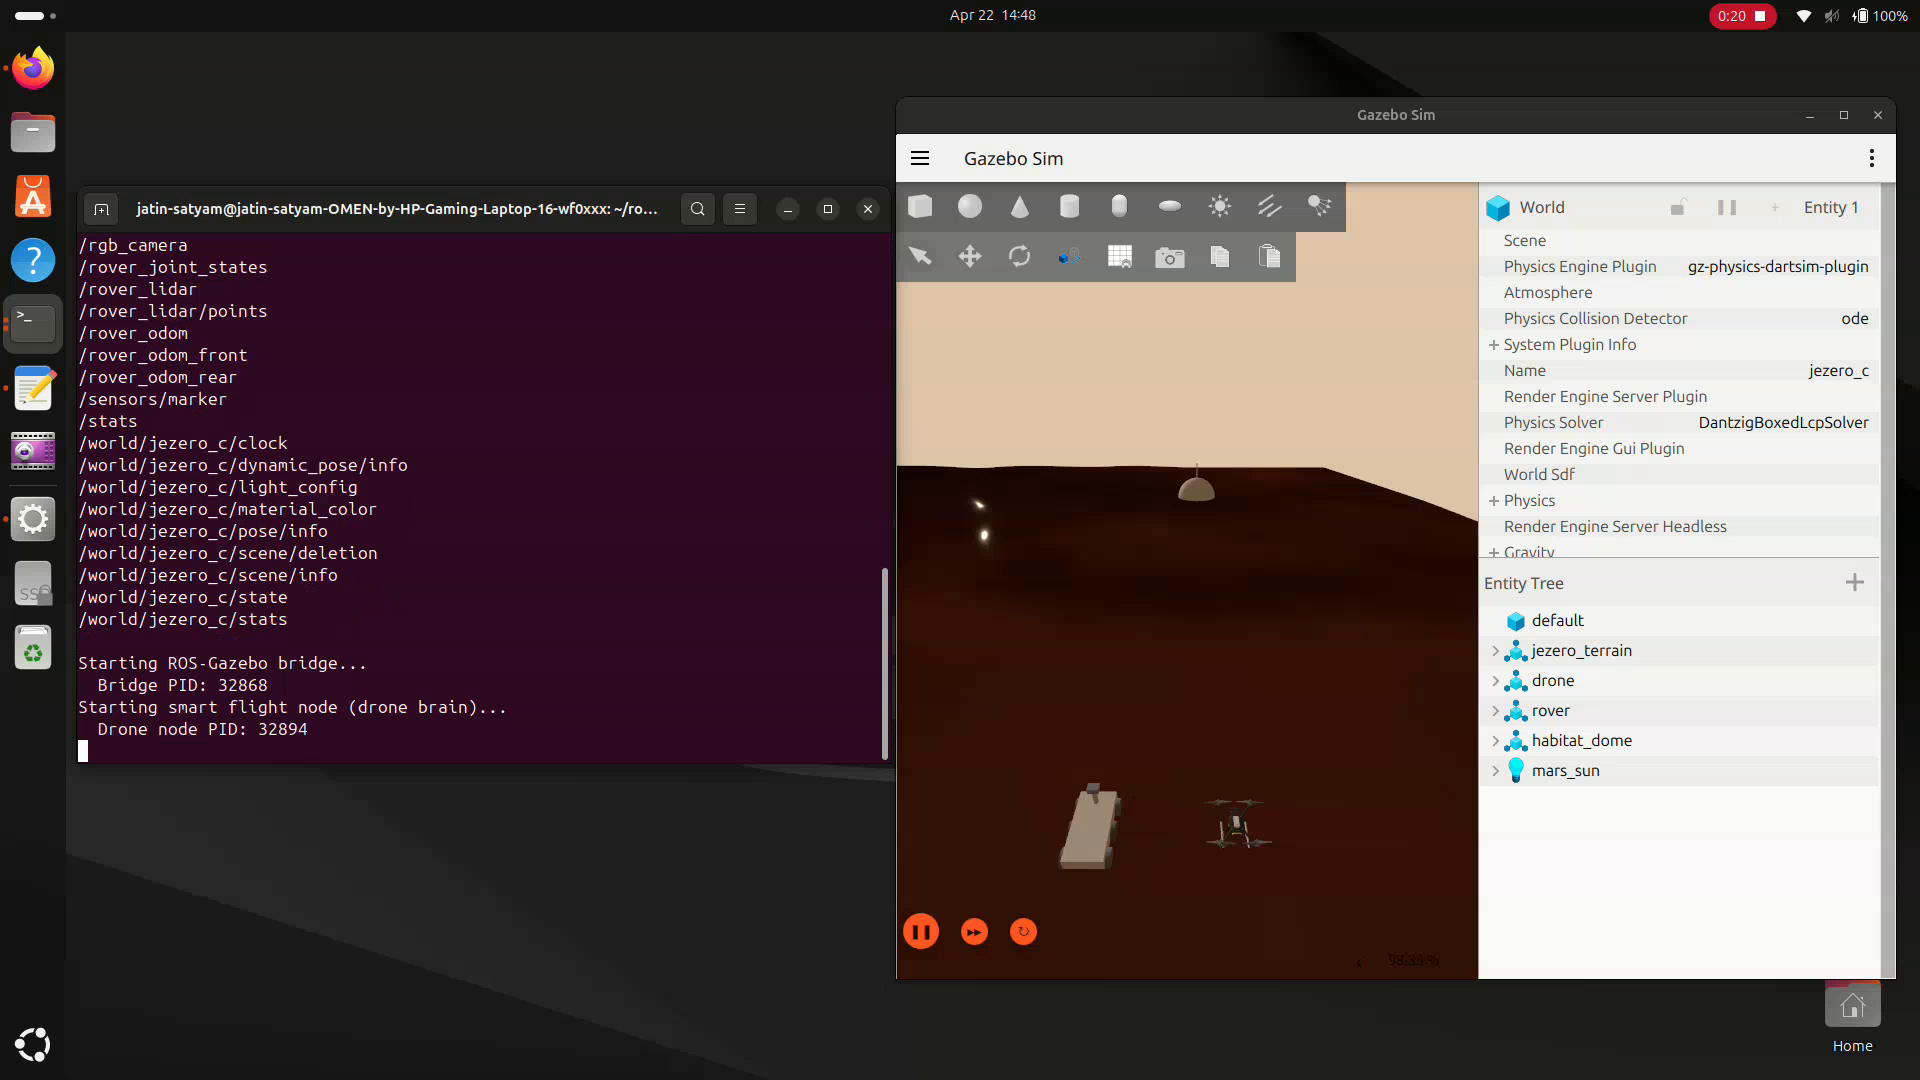
\includegraphics[width=\columnwidth]{figures/sim_gazebo_overview.png}
\caption{Gazebo Harmonic simulation at mission start: X500 drone (right) and Mars rover (left) on the HiRISE-derived Jezero Crater terrain. The terminal shows the ROS-Gazebo bridge and \texttt{smart\_flight\_node} initialising.}
\label{fig:sim_overview}
\end{figure}

\subsection{ROS2 Node Architecture and Mission Execution}
Three ROS2 Jazzy nodes coordinate the cooperative mission. The \texttt{smart\_flight\_node} commands the drone through a 10-waypoint lawnmower survey at 8\,m AGL, capturing depth and RGB frames at each keyframe, then lands autonomously. The \texttt{smart\_rover\_node} waits for the drone's occupancy grid, runs A* path planning to the habitat dome across 18 computed waypoints, and handles real-time obstacle avoidance. The \texttt{trn\_node} (Terrain-Relative Navigation) fuses scan-to-map matching against the drone's aerial map to produce pose corrections for the rover. Fig.~\ref{fig:sim_running} shows the terminal at the moment all systems are active: the drone reports \texttt{TAKEOFF complete -- starting SURVEY (10 waypoints)} while the rover initialises and waits for the occupancy grid.

\begin{figure}[t]
\centering
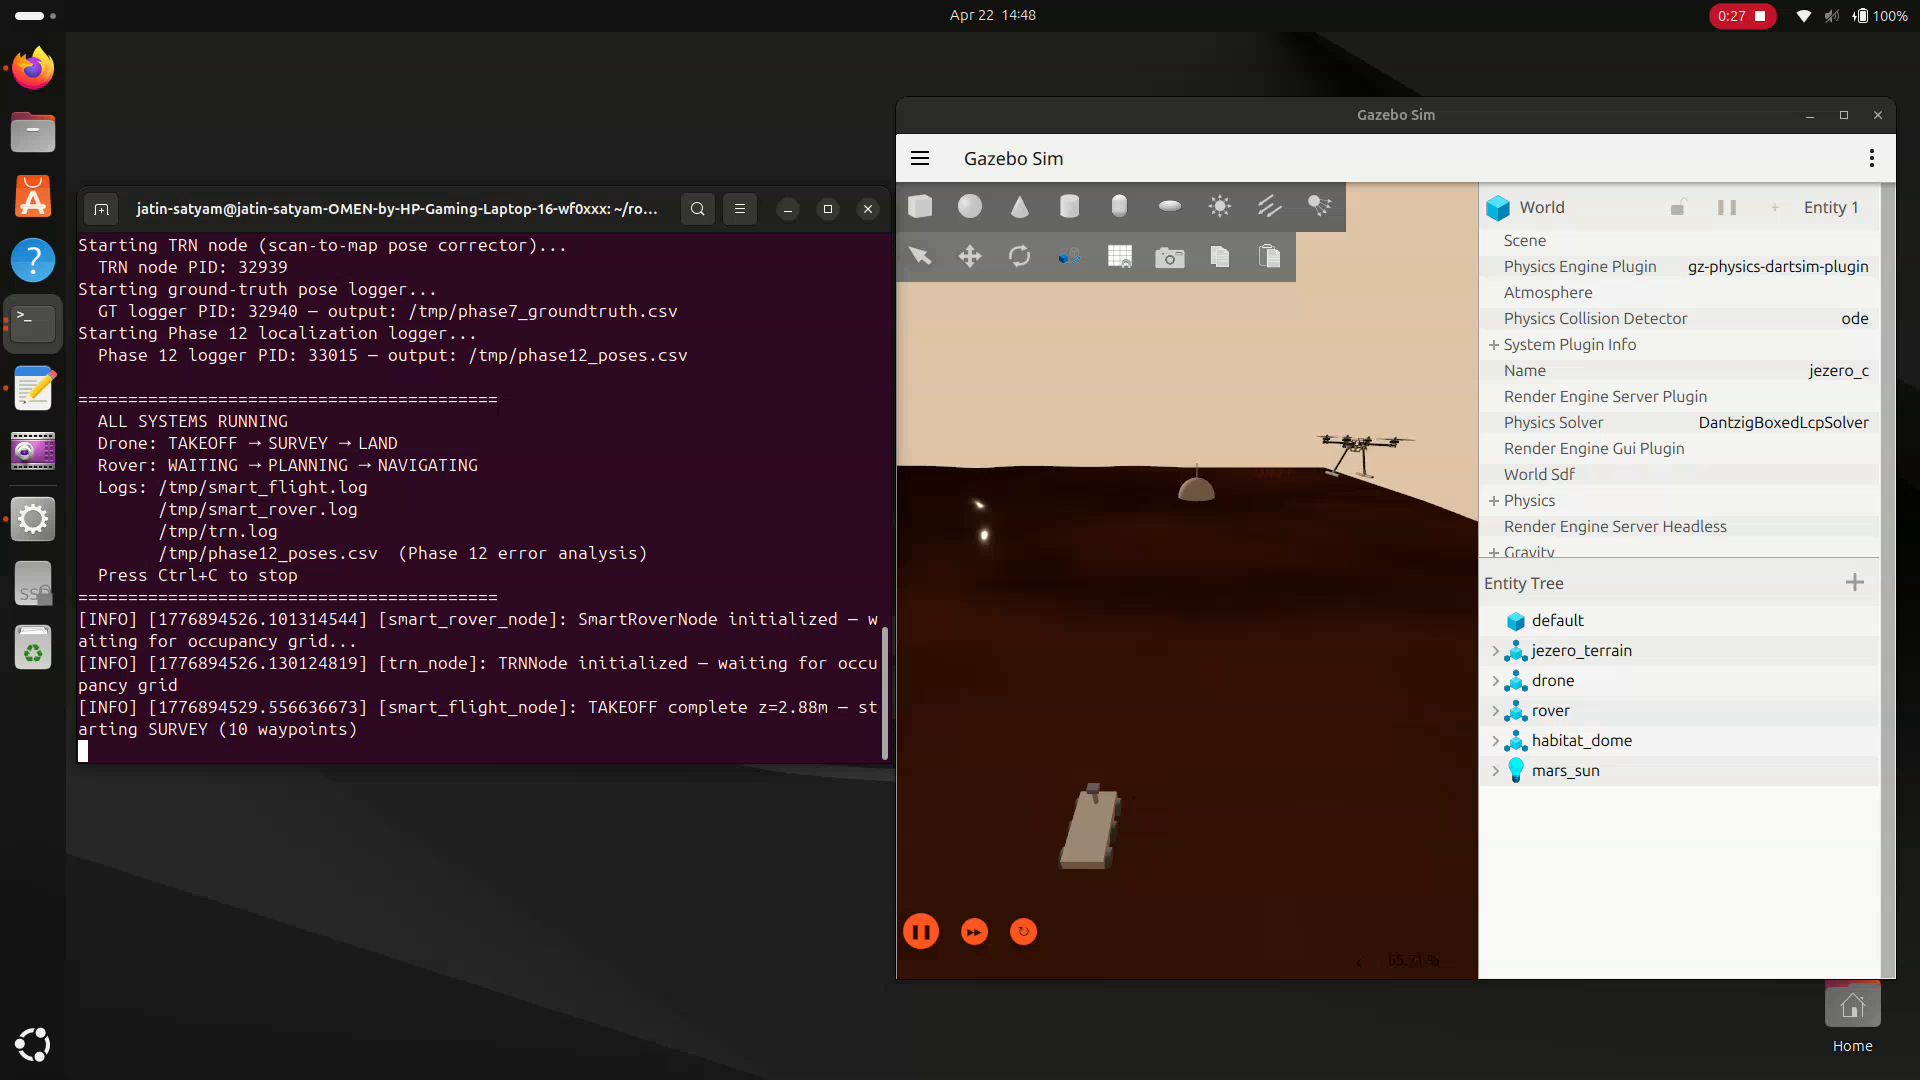
\includegraphics[width=\columnwidth]{figures/sim_running.png}
\caption{All systems running: \texttt{smart\_flight\_node} completes takeoff and begins the 10-waypoint survey; \texttt{smart\_rover\_node} and \texttt{trn\_node} initialise concurrently. Drone is visible over the terrain in the Gazebo window.}
\label{fig:sim_running}
\end{figure}

\subsection{Connection to the 3DGS Pilot}
The frames captured during the drone's lawnmower survey are the direct input to the offline reconstruction pipeline in Section~VI-A. COLMAP registers the frames into a sparse point cloud; Nerfstudio's splatfacto trainer produces the approximately 14{,}000 Gaussian field used in the pilot experiment. The per-Gaussian uncertainty pattern in Fig.~\ref{fig:uncertainty} therefore reflects the actual coverage geometry of the simulated survey: terrain edges and turn-around zones receive fewer observation angles, producing the higher-uncertainty periphery visible in that figure. The rover trajectory used in the path-conditioned gain evaluation is drawn from the same A* plan the \texttt{smart\_rover\_node} computed, ensuring the path-conditioning reflects a realistic mission route rather than an arbitrary hand-drawn line. The mission concludes with the rover arriving at the habitat dome; Fig.~\ref{fig:sim_complete} shows the terminal output confirming waypoint 18/18 reached, 0.73\,m from dome center.

\begin{figure}[t]
\centering
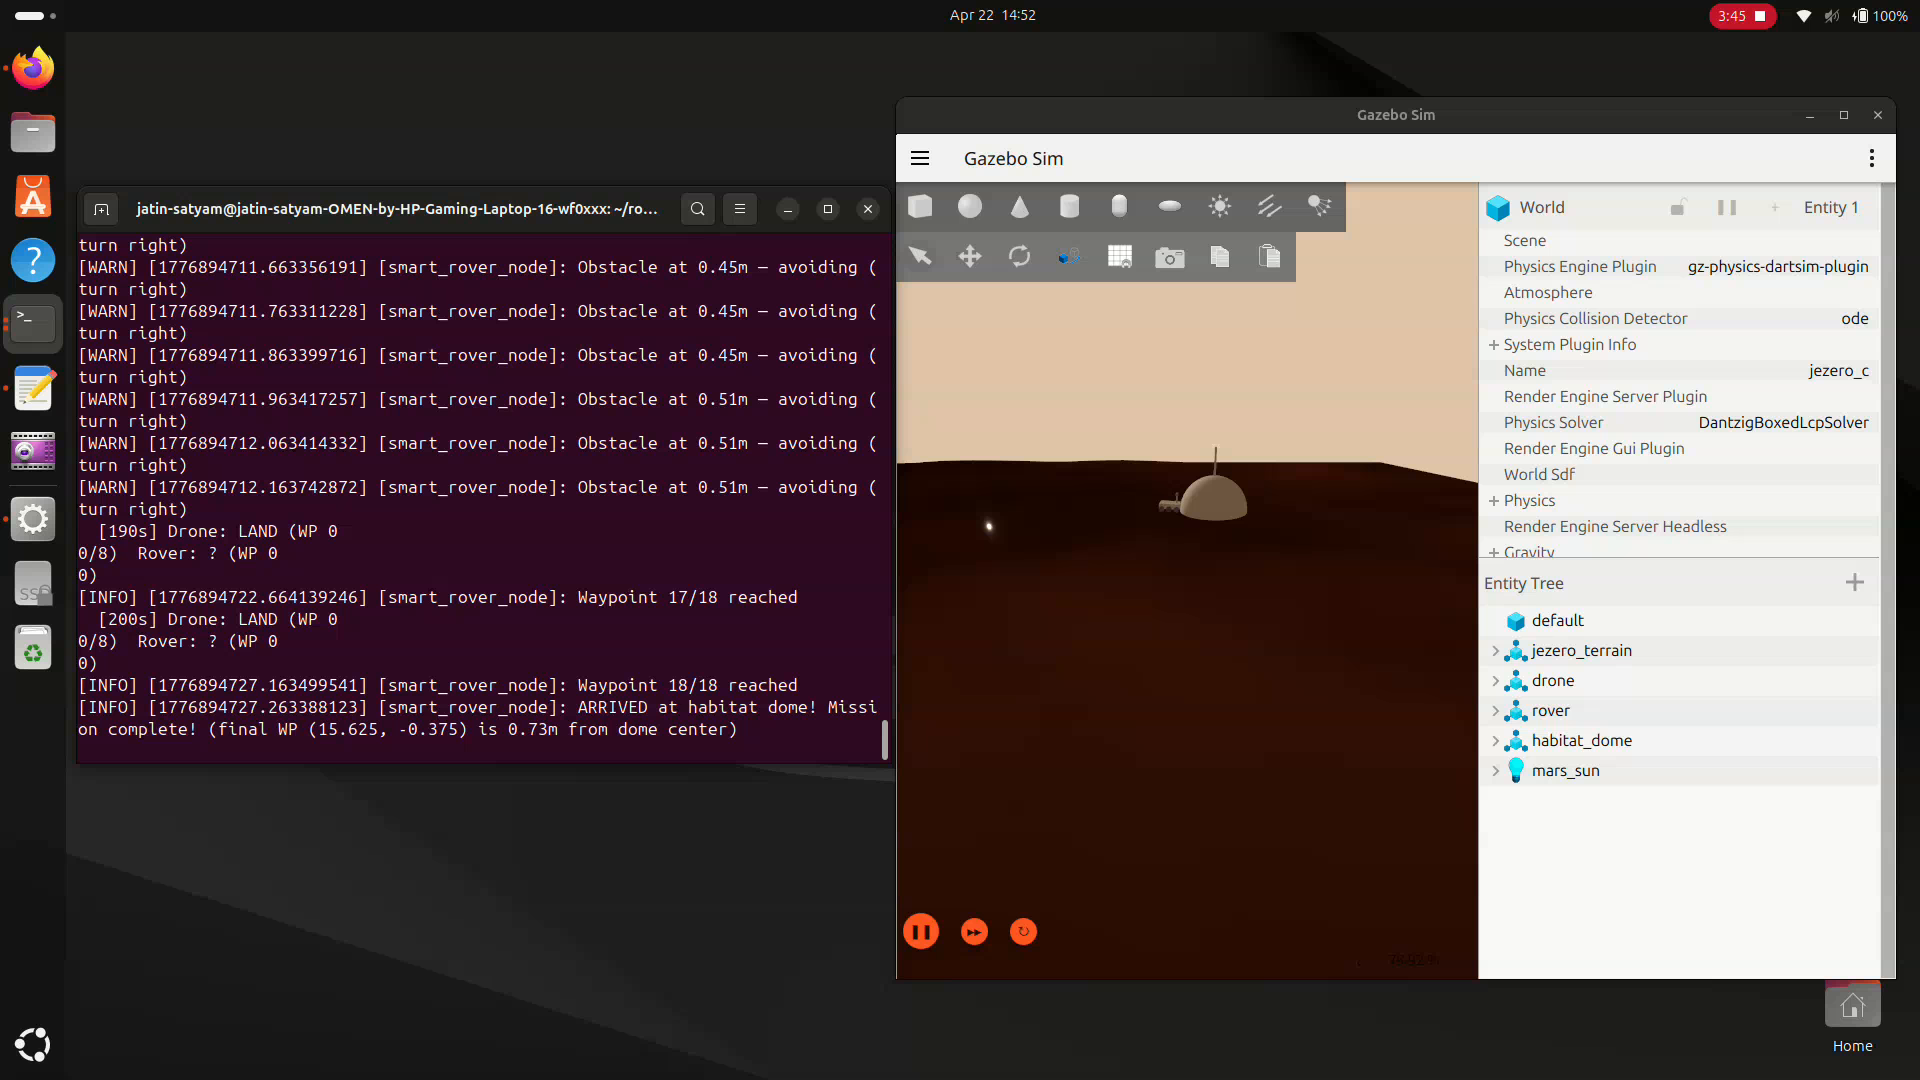
\includegraphics[width=\columnwidth]{figures/sim_complete.png}
\caption{Mission complete: \texttt{smart\_rover\_node} confirms waypoint 18/18 reached and arrival at the habitat dome (0.73\,m from dome center) after navigating around rock obstacles using the drone-supplied occupancy map.}
\label{fig:sim_complete}
\end{figure}

\subsection{Path to Real Deployment via PX4 Autopilot}
The simulation is architected to minimise the gap to real hardware. The drone control layer communicates with PX4 SITL via uXRCE-DDS -- the same bridge used in PX4's production hardware stack. Transitioning to a physical X500 with a Pixhawk 6C requires replacing the SITL binary with the hardware flight controller running PX4 v1.14+, preserving the same DDS namespace and \texttt{mission\_config.yaml} parameters. The \texttt{smart\_flight\_node}'s Offboard mode command sequence -- arming, 10\,Hz TrajectorySetpoint publishing with correct NaN velocity fields -- is identical between SITL and hardware. The \texttt{smart\_rover\_node} and \texttt{trn\_node} are hardware-agnostic ROS2 nodes requiring only a Nav2-compatible odometry source on the physical rover. The remaining integration work is sensor calibration (depth camera intrinsics for COLMAP, TRN scan-matching threshold tuning) and a field survey of a planetary-analog site to seed the initial 3DGS field. These are standard steps, not architectural changes, and represent a credible path to the field deployment that future work should pursue.


\section{Limitations}
We are explicit about what this pilot does and does not show.

The system is sim-only. ActiveGS, Traversing Mars, Splat-Nav, and LSRC have all been demonstrated on real hardware, with LSRC specifically at planetary-analog field sites. A reviewer's first question about real hardware is the expected push-back, not a possible one. We treat this as future work in Section IX rather than dismissing the concern.

The 3DGS reconstruction is offline. The streaming front-end discussed in Section IV-B is not implemented. The pilot uses a single static reconstruction rather than an online incremental one, which means the system cannot demonstrate the closed-loop behaviour where the drone's view-selection iteratively refines the field that the rover is reading from.

The rover trajectory is a single fixed plan rather than a probabilistic distribution over plans. RaEM's masking handles a single waypoint sequence; our soft prior does too, by construction. Extending to a distribution over plans (relevant when the rover's planner is itself uncertainty-aware and produces multiple candidates) is a natural extension but is not exercised here.

The per-Gaussian uncertainty proxy is weak. Covisibility count and opacity are usable proxies but they are not calibrated probabilistic uncertainties. Methods like Predictive Photometric Uncertainty would be sharper but require a separate calibration step that is out of scope for the pilot. We note in Section IV-C that the upgrade is plug-and-play.

The traversability semantics are themselves a simplification. A field-deployed system would need a slip / wheel-cost model that responds to terrain mechanics. Endo et al. and LSRC both demonstrate what production-grade traversability looks like; the pilot uses geometric proxies as a stand-in.

\section{Future Work}
The full implementation has been described in Section IV. The path from the pilot to the full system has several sub-steps. The streaming 3DGS front-end needs to be selected (MonoGS, MASt3R, or hybrid) and benchmarked on the project's RTX 4060. The per-Gaussian uncertainty layer needs to be upgraded to a calibrated estimator, probably Predictive Photometric Uncertainty for plug-and-play behaviour. The NBV planner needs to be wrapped in a ROS2 node and integrated with the existing drone control loop. The traversability projection layer needs slip semantics rather than geometric proxies. The rover's planner needs the wait-for-more-info option wired in. The drone-rover communication interface needs an actual message specification.

A real-hardware demonstration is the natural follow-up. A small drone (Crazyflie or Tello-class) and a small wheeled rover (TurtleBot or equivalent) on textured foam terrain on a tabletop is a feasible scope. Real-hardware validation is the right way to address the most likely reviewer push-back about whether the simulation results transfer.

A multi-drone extension is the second natural follow-up. Traversing Mars is single-scout. MAP-NBV \cite{mapnbv} provides a pre-3DGS multi-agent NBV reference. The cooperative aerial-aerial-ground variant is the obvious next-step.

The cluster of work this paper specialises has been publishing every four to six months. We expect that within a year there will be additional published methods that close adjacent pieces of the gap, and the surviving novel contribution may need to be re-articulated against the new work.

\section{Conclusion}
This paper presents a path-conditioned next-best-view formulation for cooperative aerial-ground Mars scouting on a 3D Gaussian Splatting substrate, framed honestly as a specialisation of recently published methods rather than as a wholesale novel integration. The gain function generalises RaEM's discrete-waypoint masking to a soft path-likelihood prior, substitutes traversability semantics for collision-risk semantics, and is the cross-agent variant of Khass's single-agent proximity-weighted Fisher gain. A pilot experiment on a HiRISE-derived 3DGS reconstruction of Jezero Crater demonstrates the formulation in a concrete setting and shows that path-conditioning meaningfully shifts viewpoint selection relative to a uniform-weight baseline. The full closed-loop system, real-hardware validation, and multi-drone extensions are the natural follow-up work.

\bibliographystyle{IEEEtran}
\bibliography{references}

\end{document}
